
\section{Experiment Overview}

% AMS-01 --> AMS-02
The Alpha Magnetic Spectrometer (AMS) experiment was proposed by Nobel laureate Prof. Samuel Ting from MIT in 1994 and was soon accepted \cite{AMSProposal1994}. The goal of the experiment is to search for antimatter and dark matter in the universe
and to provide precise measurements of the fluxes for different components of the cosmic rays, which is crucial for understanding the sources of cosmic rays and their basic propagation model \cite{AMS02Goal}. \par

To test the feasibility of a particle spectrometer in space, a prototype called AMS-01 (figure \ref{AMS01Detector}) was designed, which was a simplified version of the final detector. The test flight was conducted in 1998 during the space shuttle mission STS-91 \cite{AMS01Result}, see figure \ref{AMS01TestFlight}. By collecting cosmic ray data for ten days, the test flight proved that placing and operating a spectrometer in space is possible.   \par
    
\begin{figure}[] 
\centering   
\subfigure[] { \label{AMS01Detector}    
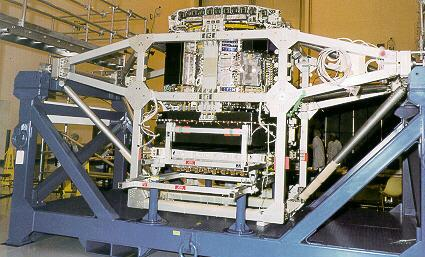
\includegraphics[width=0.5\textwidth, height=0.3\textheight]{Figures/chapter3/Overview/AMS01Detector.jpg}    
}    
\subfigure[] { \label{AMS01TestFlight}    
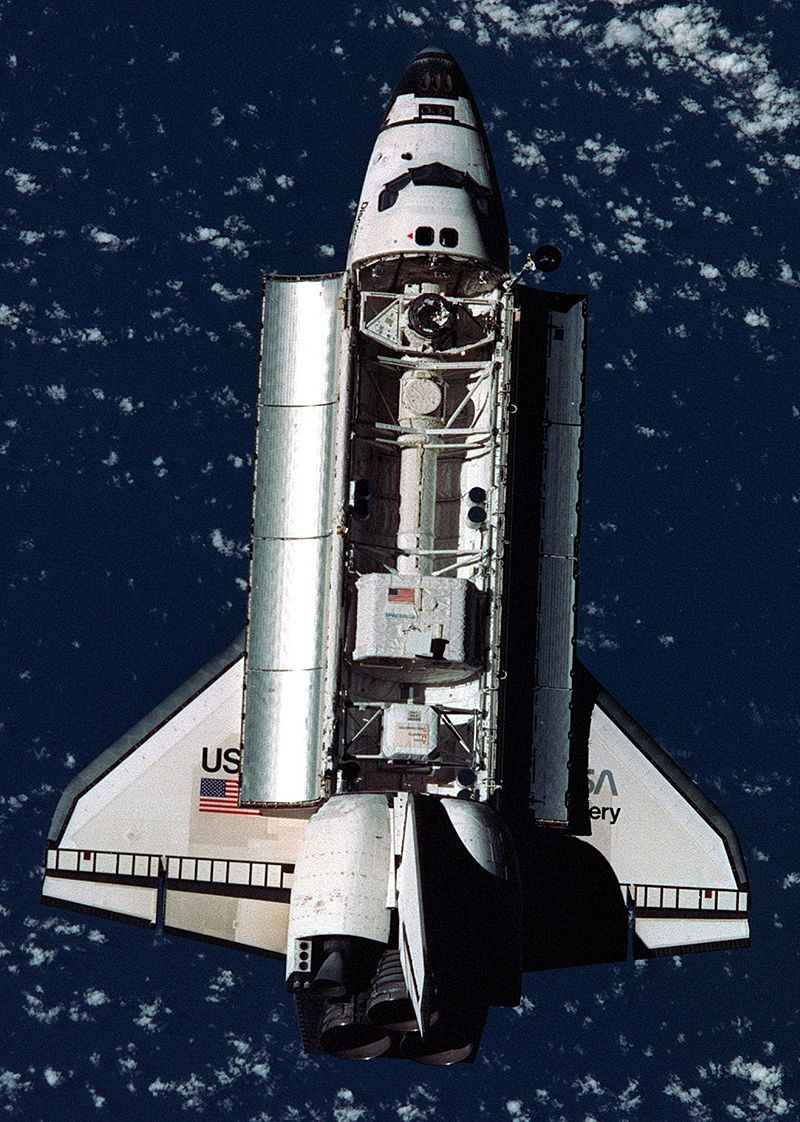
\includegraphics[width=0.4\textwidth, height=0.37\textheight]{Figures/chapter3/Overview/AMS-01.jpg} 
}    
\caption[The AMS-01 detector.]{a) The AMS-01 detector at the Kennedy Space Center (NASA) with its support structure \cite{AMS01Brochure}; b) The AMS-01 detector aboard the Space Shuttle Discovery during the STS-91 mission in June 1998 \cite{WikiAMS01Flight}.}   
    
\label{AMS01}    
\end{figure}

After several years of construction and testing, the AMS-02 detector was launched aboard the space shuttle Endeavour during mission STS 134 from Kennedy Space Center on 16 May 2011. Three days later, the detector was installed on the ISS's S3 Upper Inboard Payload Attach Site and began collecting data. Figure \ref{AMS02OnISS} shows the location of AMS-02 on the ISS. \par

\begin{figure}[]
\centering
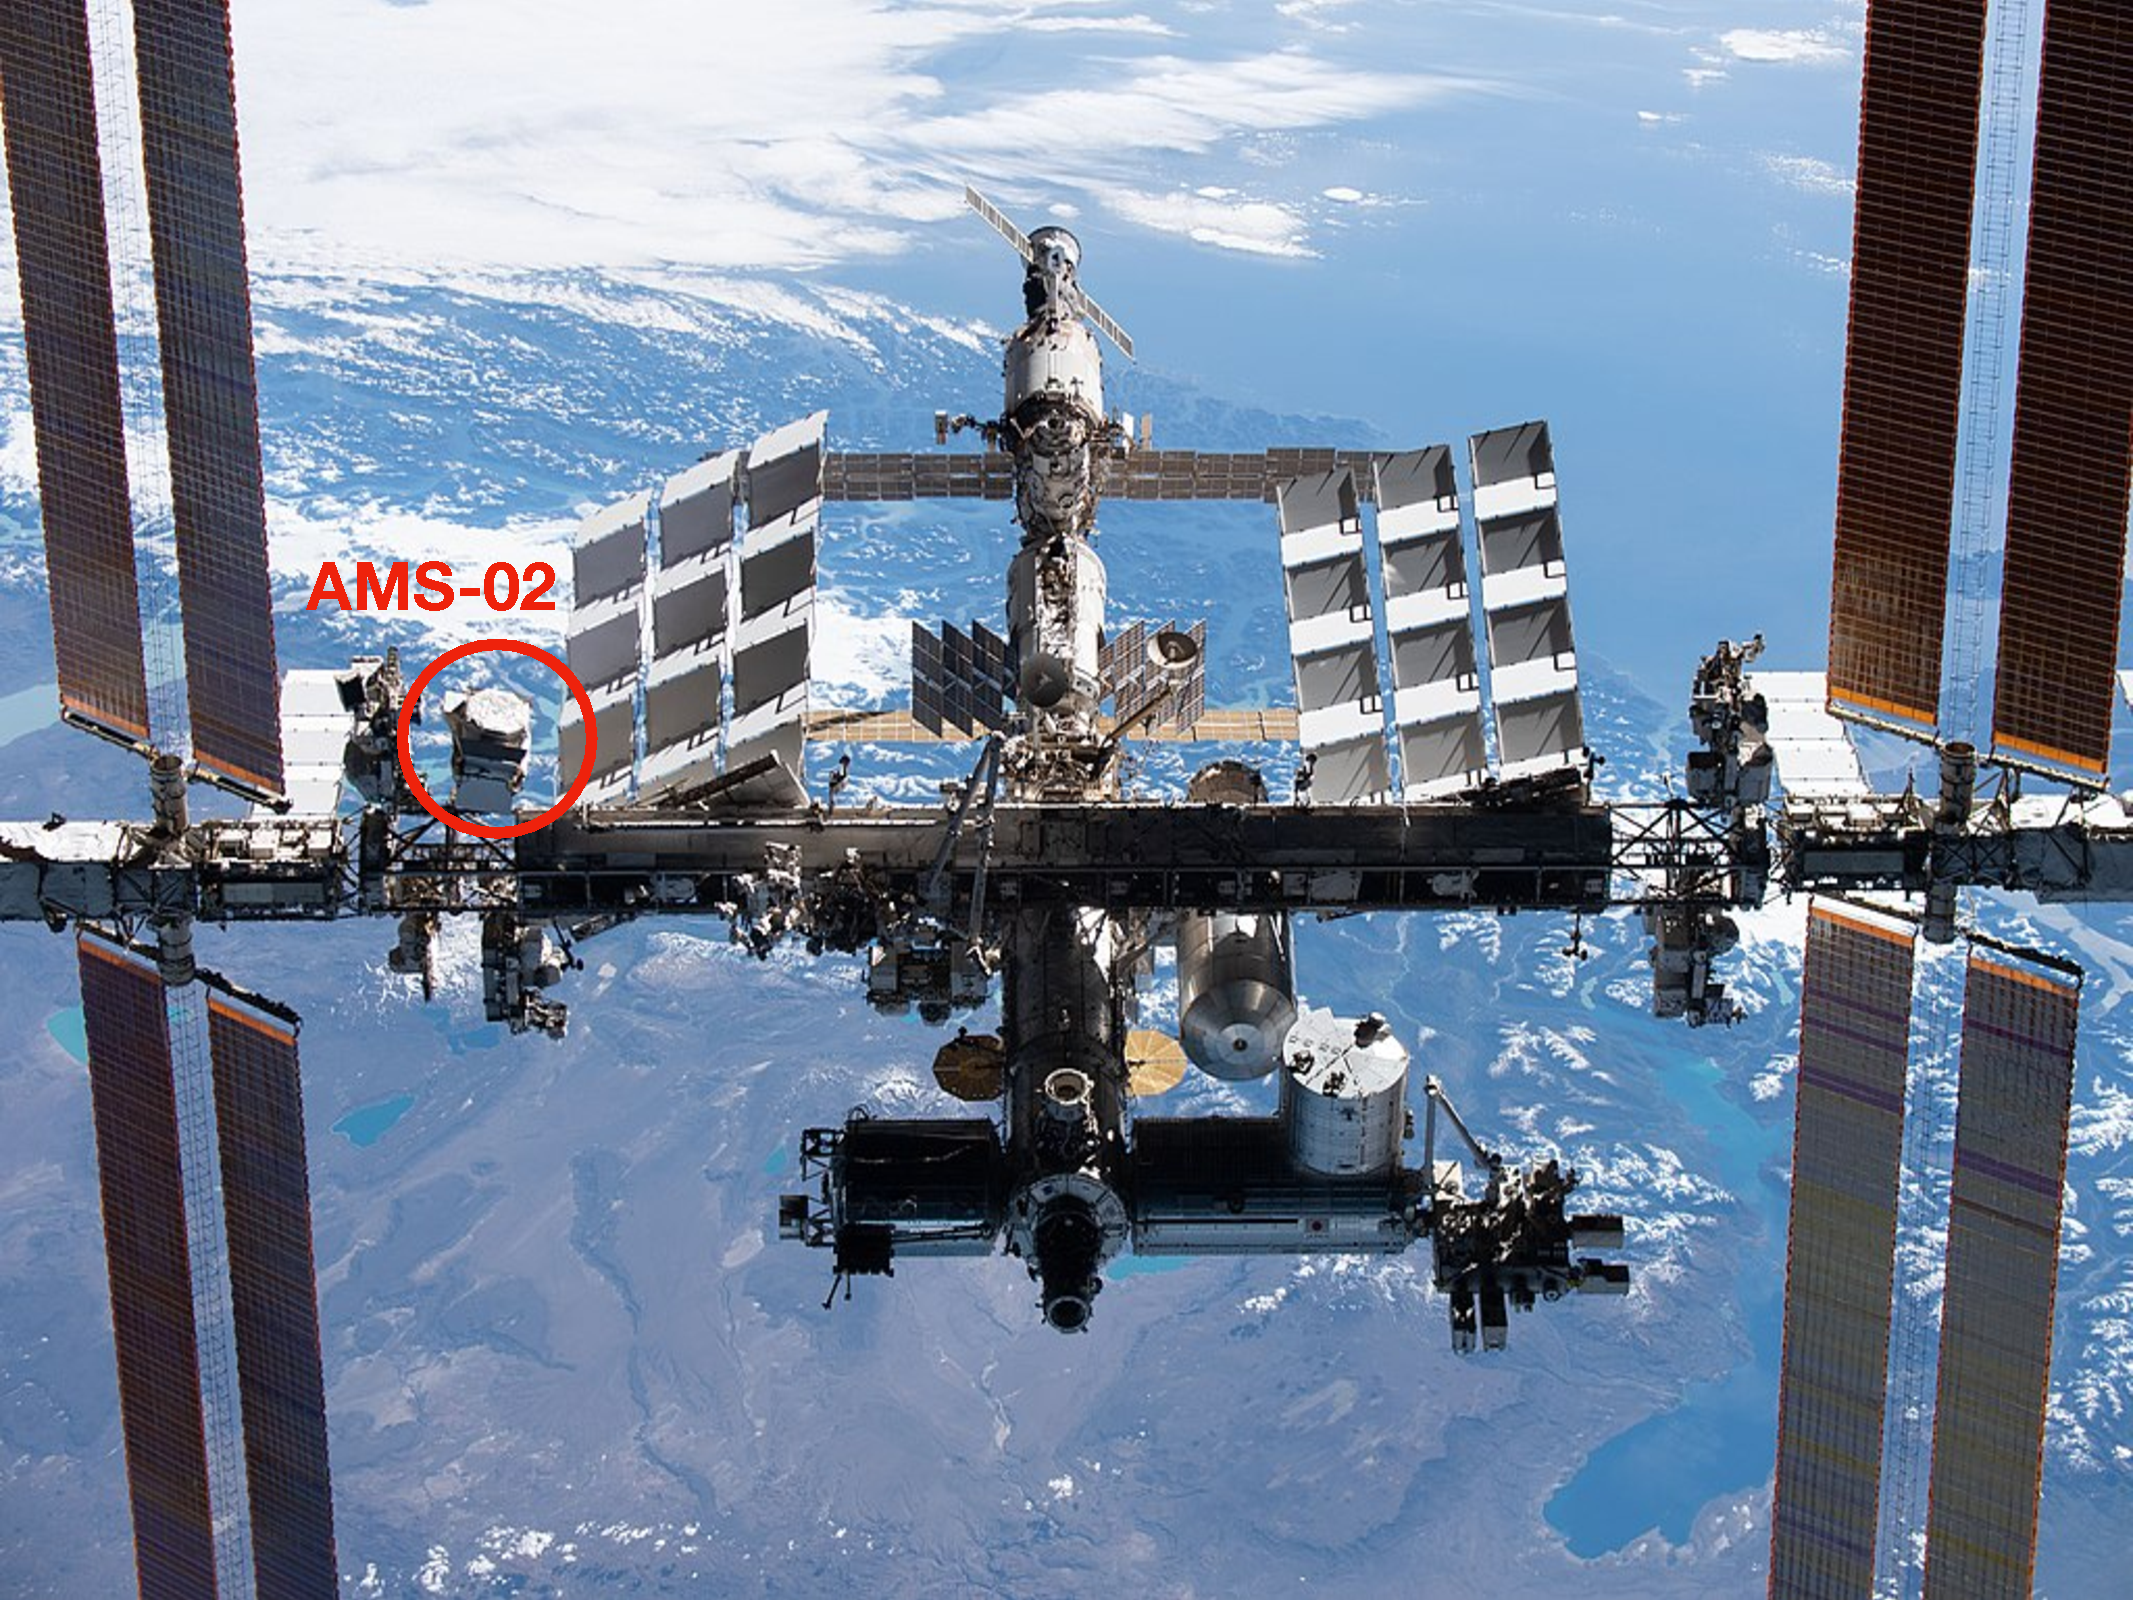
\includegraphics[width=0.8\textwidth, height=0.39\textheight ]{Figures/chapter3/Overview/AMS02OnISS.pdf}
\caption[The AMS-02 detector on the ISS.]{The AMS-02 detector mounted on the ISS S3 Upper Inboard Payload Attach Site (Image modified from \cite{wikiISS}). }
\label{AMS02OnISS}
\end{figure}

% Sub-detectors
The AMS-02 detector has a size of 5 m $\times$ 4 m $\times$ 3 m and weighs 7.5 t \cite{PhysicsReport2}. It has a permanent magnet that provides a magnetic field of 0.14 T and in combination with nine silicon tracker layers the rigidity of the cosmic particles can be measured. Within the magnet, the Anti-Coincidence Counters (ACC) are used as a veto system to reject particles entering the detector sideways. At the top of the experiment, there is a Transition Radiation Detector (TRD), which can distinguish light and heavy particles. Above and below the magnet there are two Time-Of-Flight (TOF) systems which provide the trigger and the measurements of the velocity and the charge of the particles. Below the lower part of the TOF, a Ring-Imaging Cherenkov (RICH) detector is located so the particle's velocity can be measured. At the bottom of the detector, there is an Electromagnetic Calorimeter (ECAL) which measures the energy of the particles. The geometry of all the sub-detectors is illustrated in figure \ref{AMS02Geometry}. 

\begin{figure}[]
\centering
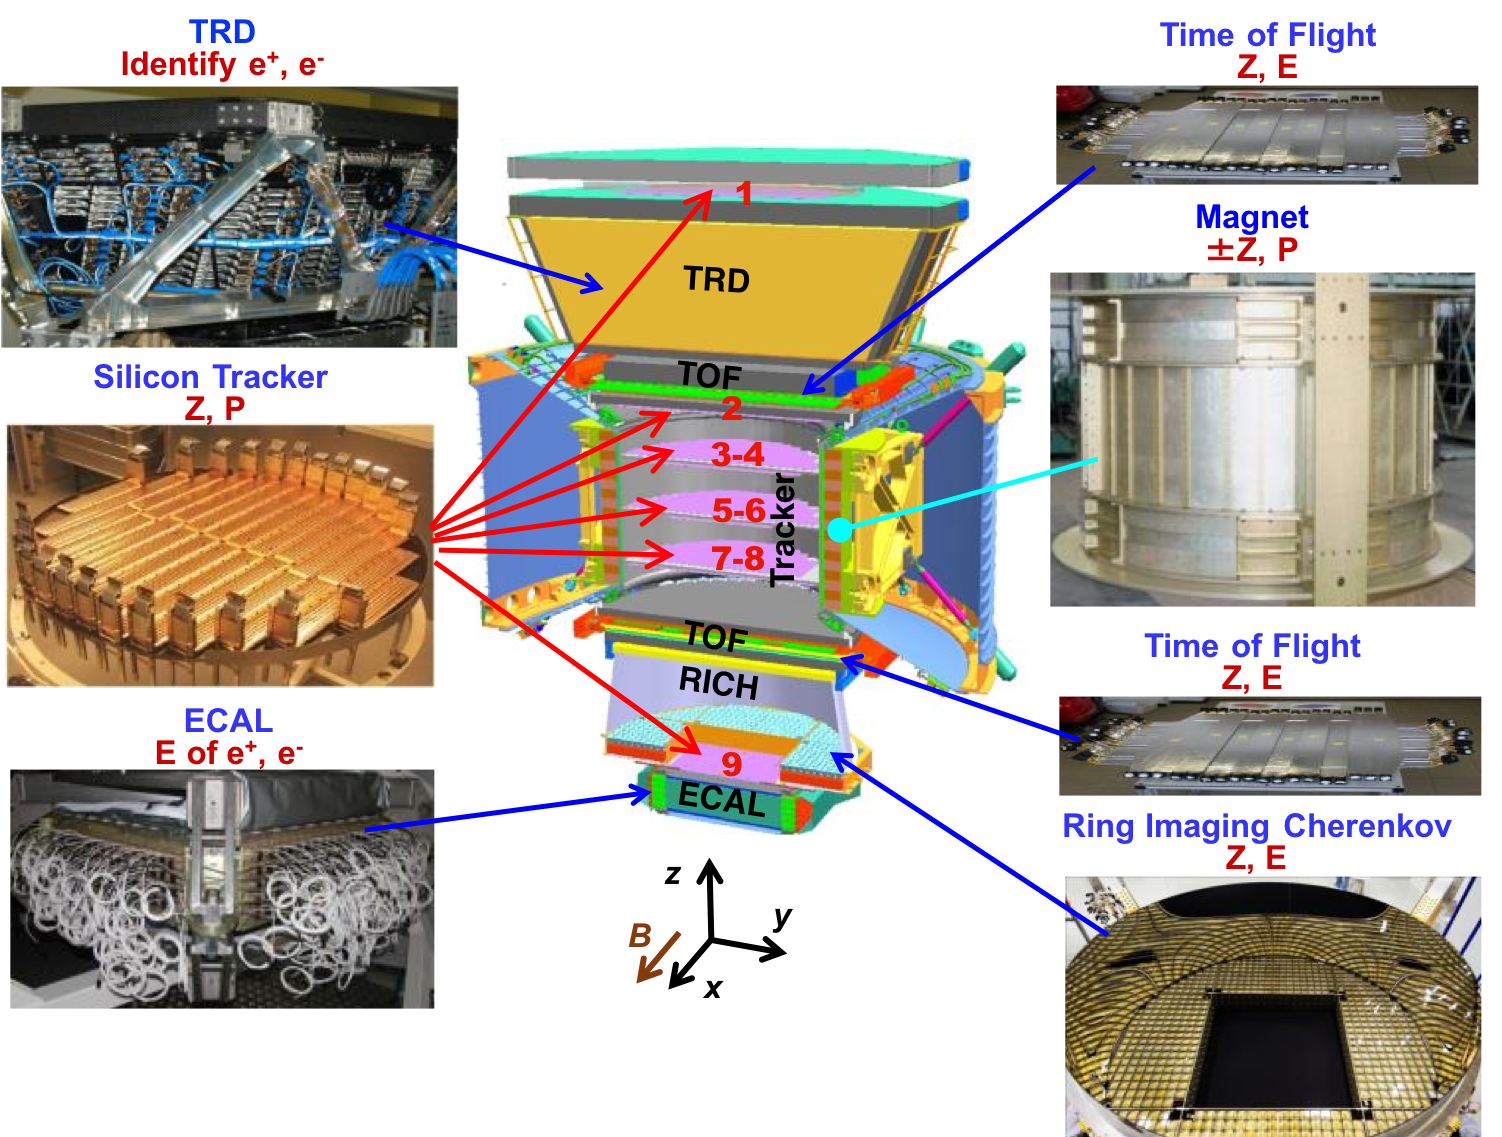
\includegraphics[width=0.8\textwidth, height=0.4\textheight ]{Figures/chapter3/Overview/AMS02Geometry.png}
\caption[Schematic view of the AMS-02 experiment.]{Schematic view of the AMS-02 experiment and all its sub-detectors \cite{AMSWebside}. }
\label{AMS02Geometry}
\end{figure}

% operations 
Detector operations have been conducted since the launch to make the experiment run smoothly. These operations can be distinguished in flight and ground operations. As part of the flight operations, the collected data is transmitted from the ISS to tracking and data relay satellites (TDRS). Then through the S (low rate) and Ku (high rate) radiofrequency bands, the data is transmitted to the White Sands Ground Terminal (WSGT) in New Mexico. Over the NASA networks, the data is then directed to the Marshall Space Flight Center (MSFC) and is written on disk. At last, the data is transmitted over the Internet and copied to the Payload Operations Control Centre (POCC) at CERN.

%The collected data is transmitted from the upper left to the lower left in this figure in a clockwise sequence. The command from the ground to the space station follows the counterclockwise sequence. In figure \ref{AMS02operations} the operation process is illustrated.
%\begin{figure}[]
%\centering
%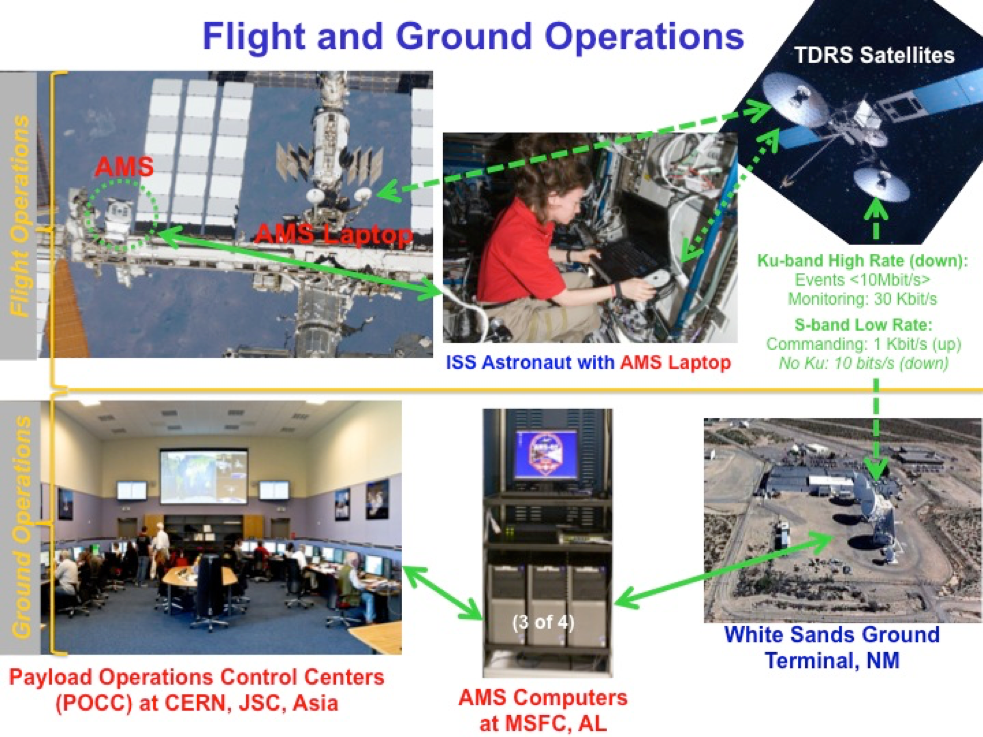
\includegraphics[width=0.8\textwidth, height=0.4\textheight ]{Figures/chapter3/Overview/Operations.png}
%\caption{A overview of AMS-02 experiment operations flow in flight and ground \cite{AMSWebside} }
%\label{AMS02operations}
%\end{figure}






